%\VignetteIndexEntry{PharmacoGx: an R package for analysis of large pharmacogenomic datasets}
%\VignetteDepends{xtable}
%\VignetteSuggests{}
%\VignetteKeywords{}
%\VignettePackage{PharmacoGx}

\documentclass[11pt]{article}

\usepackage[utf8]{inputenc}
\usepackage{authblk}


\title{PharmacoGx: an R package for analysis of large pharmacogenomic datasets}
\author[1]{Petr Smirnov}
\author[1,2]{Zhaleh Safikhani}
%\author[1]{Mark Freeman}
\author[1,2]{Benjamin Haibe-Kains}
\affil[1]{Princess Margaret Cancer Centre, University Health Network, Toronto Canada}
\affil[2]{Department of Medical Biophysics, University of Toronto, Toronto Canada}




\usepackage{Sweave}
\begin{document}
\Sconcordance{concordance:PharmacoGx.tex:/home/chris/rPackages/PharmacoGx/vignettes/PharmacoGx.Rnw:%
1 21 1 1 4 1 1 1 0 69 1 1 3 2 0 1 1 3 0 1 2 1 1 1 2 4 0 1 2 12 1 1 3 2 %
0 1 1 3 0 1 2 5 1 1 3 5 0 1 2 16 1 1 2 1 0 3 1 1 2 1 0 1 3 2 0 1 7 4 0 %
1 5 4 0 1 6 4 0 1 5 4 0 1 6 4 0 1 5 4 0 2 1 1 5 3 0 1 4 3 0 1 4 3 0 1 3 %
1 0 1 2 1 0 1 1 1 2 1 0 1 10 13 0 1 3 2 1 1 -5 1 12 13 1 1 2 1 0 2 1 1 %
3 2 0 1 1 1 7 5 0 1 2 2 1 1 2 20 0 1 2 45 1 1 3 1 0 1 3 2 0 1 8 7 0 1 8 %
7 0 4 1 16 0 1 2 51 1 1 2 31 0 1 2 4 1}


\maketitle
\tableofcontents

%------------------------------------------------------------
\section{Introduction}
%------------------------------------------------------------

Pharmacogenomics holds much potential to aid in discovering drug response
biomarkers and developing novel targeted therapies, leading to development of
precision medicine and working towards the goal of personalized therapy.
Several large experiments have been conducted, both to molecularly
characterize drug dose response across many cell lines, and to examine the
molecular response to drug administration. However, the experiments lack a
standardization of protocols and annotations, hindering meta-analysis across
several experiments.\\

\textit{PharmacoGx} was developed to address these challenges, by providing a
unified framework for downloading and analyzing large pharmacogenomic datasets
which are extensively curated to ensure maximum overlap and consistency.
\textit{PharmacoGx} is based on a level of abstraction from the raw
experimental data, and allows bioinformaticians and biologists to work with
data at the level of genes, drugs and cell lines. This provides a more
intuitive interface and, in combination with unified curation, simplifies
analyses between multiple datasets.\\

To organize the data released by each experiment, we developed the
\textit{PharmacoSet} class. This class efficiently stores different types of
data and facilitates interrogating the data by drug or cell line. The
\textit{PharmacoSet} is also versatile in its ability to deal with two
distinct types of pharmacogenomic datasets. The first type, known as
\textit{sensitivity} datasets, are datasets where cell lines were profiled
on the molecular level, and then tested for drug dose response. The second
type of dataset is the \textit{perturbation} dataset. These types of
datasets profile a cell line on the molecular level before and after
administration of a compound, to characterize the action of the compound on
the molecular level.\\

With the first release of \textit{PharmacoGx} we have fully curated and
created PharmacoSet objects for three publicly available large pharmacogenomic
datasets. Two of these datasets are of the \textit{sensitivity} type. These
are the Genomics of Drug Sensitivity in Cancer Project (GDSC) \cite{garnett_systematic_2012} and the Cancer 
Cell Line Encyclopedia (CCLE) \cite{barretina_cancer_2012}. The third dataset is of the
\textit{perturbation} type, the Connectivity Map (CMAP) project
\cite{lamb_connectivity_2006}.\\

Furthermore, PharmacoGx provides a suite of parallized functions which
facilitate drug response biomarker discovery, and molecular drug
characterization. This vignette will provide two example analysis case
studies. The first will be comparing gene expression and drug sensitivity
measures across the CCLE and GDSC projects. The second case study will
interrogate the CMAP database with a known signature of up and down regulated
genes for HDAC inhibitors as published in ~\cite{glaser_gene_2003}. Using the
Connectivity Score as defined in ~\cite{lamb_connectivity_2006}, it will be seen that
known HDAC inhibitors have a high numerical score and high significance.\\ 

For the purpose of this vignette, an extremely minuscule subset of all three
\textit{PharmacoSet} objects are included with the package as example data.
They are included for illustrative purposes only, and the results obtained
with them will likely be meaningless.\\


%------------------------------------------------------------
\subsection{Installation and Settings}
%------------------------------------------------------------

\textit{PharmacoGx} requires that several packages are installed. However, all dependencies are available from CRAN or Bioconductor.

\begin{Schunk}
\begin{Sinput}
> source('http://bioconductor.org/biocLite.R')
> biocLite('PharmacoGx')
\end{Sinput}
\end{Schunk}

Load \textit{PharamacoGx} into your current workspace:
\begin{Schunk}
\begin{Sinput}
> library(PharmacoGx)
\end{Sinput}
\end{Schunk}

%------------------------------------------------------------
\subsection*{Requirements}
%------------------------------------------------------------

\textit{PharmacoGx} has been tested on Windows, Mac and Cent OS platforms. The packages uses the core R package \textit{parallel} to preform parallel computations, and therefore if parallelization is desired, the dependencies for the parallel package must be met. 

%------------------------------------------------------------
\section{Downloading PharmacoSet objects}
%------------------------------------------------------------

We have made the PharmacoSet objects of the curated datasets available online at:\\ \textit{www.pmgenomics.ca/bhklab/software/pharmacogx/}\\

However, to make the process of obtaining the data easier through the R shell, we have also written a function \textit{downloadPSet} which automates downloading the datasets into a directory of the users choice, and returns the data into the R session. 

\begin{Schunk}
\begin{Sinput}
> ## Example
> GDSC <- downloadPSet("GDSC") 
\end{Sinput}
\end{Schunk}
%------------------------------------------------------------
\subsection*{Downloading Drug Signatures}
%------------------------------------------------------------

The package also provides tools to compute drug perturbation and sensitivity signatures, as explained below. However, the computation of the perturbation signatures is very lengthy, so for users' convenience we have precomputed the signatures for our perturbation PharmacoSet objects and made them available for download using the function \textit{downloadPertSig}.

\begin{Schunk}
\begin{Sinput}
> ## Example
> CMAP.sigs <- downloadPertSig("CMAP")
\end{Sinput}
\end{Schunk}

%------------------------------------------------------------
\section{Case Study}
%------------------------------------------------------------

%------------------------------------------------------------
\subsection{(In)Consistency across large pharmacogenomic studies}
%------------------------------------------------------------
Our first case study illustrates the functions for analysis of the \textit{sensitivity} type of dataset. The case study will investigate the consistency between the GDSC and CCLE datasets, recreating the analysis similar to our \textit{Inconsistency in Large Pharmacogenomic Studies} paper \cite{haibe-kains_inconsistency_2013}. In both CCLE and GDSC, the transcriptome of cells was profiled using an Affymatrix microarray chip. Cells were also tested for their response to increasing concentrations of various compounds, and form this the IC50 and AUC were computed. However, the cell and drugs names used between the two datasets were not consistent. Furthermore, two different microarray platforms were used. However, \textit{PharmacoGx} allows us to overcome these differences to do a comparative study between these two datasets. \\


GDSC was profiled using the hgu133a platform, while CCLE was profiled with the expanded hgu133plus2 platform. While in this case the hgu133a is almost a strict subset of hgu133plus2 platform, the expression information in \textit{PharmacoSet} objects is summarized by Ensemble Gene Ids, allowing datasets with different platforms to be directly compared. The probe to gene mapping is done using the BrainArray customCDF for each platform \cite{sabatti_thresholding_2002}.

To begin, you would load the datasets from disk or download them using the \textit{downloadPSet} function above. 

\begin{Schunk}
\begin{Sinput}
>   ##Using the included example datasets
>   library(PharmacoGx)
>   data("GDSCsmall")
>   data("CCLEsmall")
\end{Sinput}
\end{Schunk}

We then want to investigate the consistency of the data between the two datasets. The common intersection between the datasets can then be found using \textit{intersectPSet}. We then create a summary of the gene expression and drug sensitivity measures for both datasets, and compare them using a standard correlation coefficient. 

\begin{Schunk}
\begin{Sinput}
>   library(Biobase)
>   library(PharmacoGx)
>   data("GDSCsmall")
>   data("CCLEsmall")
>   commonGenes <- intersect(featureNames(GDSCsmall, "rna"),
+                            featureNames(CCLEsmall,"rna"))
>   common <- intersectPSet(list('CCLE'=CCLEsmall,
+                                'GDSC'=GDSCsmall),
+                           intersectOn=c("cell.lines", "drugs"))
>   GDSC.auc <- summarizeSensitivityProfiles(
+                 common$GDSC,
+                 sensitivity.measure='auc_published', 
+                 summary.stat="median")
>   CCLE.auc <- summarizeSensitivityProfiles(
+                 common$CCLE,
+                 sensitivity.measure='auc_published', 
+                 summary.stat="median")
>   GDSC.ic50 <- summarizeSensitivityProfiles(
+                 common$GDSC, 
+                 sensitivity.measure='ic50_published', 
+                 summary.stat="median")
>   CCLE.ic50 <- summarizeSensitivityProfiles(
+                 common$CCLE, 
+                 sensitivity.measure='ic50_published', 
+                 summary.stat="median")
>   GDSCexpression <- summarizeMolecularProfiles(common$GDSC, 
+                                         cellNames(common$GDSC),
+                                         mDataType="rna",
+                                         features=commonGenes,
+                                         verbose=FALSE)
>   CCLEexpression <- summarizeMolecularProfiles(common$CCLE, 
+                                          cellNames(common$CCLE),
+                                          mDataType="rna",
+                                          features=commonGenes,
+                                          verbose=FALSE)
>   gg <- featureNames(common[[1]], 'rna')
>   cc <- cellNames(common[[1]])
>   ge.cor <- sapply(cc, function (x, d1, d2) {
+     return (stats::cor(d1[ , x], d2[ , x], method="spearman",
+                 use="pairwise.complete.obs"))
+   }, d1=exprs(GDSCexpression), d2=exprs(CCLEexpression))
>   ic50.cor <- sapply(cc, function (x, d1, d2) {
+     return (stats::cor(d1[, x], d2[ , x], method="spearman",
+                 use="pairwise.complete.obs"))
+   }, d1=GDSC.ic50, d2=CCLE.ic50)
>   auc.cor <- sapply(cc, function (x, d1, d2) {
+     return (stats::cor(d1[ , x], d2[ , x], method="spearman",
+                 use="pairwise.complete.obs"))
+   }, d1=GDSC.auc, d2=CCLE.auc)
>   w1 <- stats::wilcox.test(x=ge.cor, y=auc.cor,
+                            conf.int=TRUE, exact=FALSE)
>   w2 <- stats::wilcox.test(x=ge.cor, y=ic50.cor,
+                            conf.int=TRUE, exact=FALSE)
>   yylim <- c(-1, 1)
>   ss <- sprintf("GE vs. AUC = %.1E\nGE vs. IC50 = %.1E",
+                 w1$p.value, w2$p.value)
>   boxplot(list("GE"=ge.cor,
+                "AUC"=auc.cor,
+                "IC50"=ic50.cor),
+           main="Concordance between cell lines",
+           ylab=expression(R[s]),
+           sub=ss,
+           ylim=yylim,
+           col="lightgrey",
+           pch=20,
+           border="black")
> 
\end{Sinput}
\end{Schunk}

\begin{figure}[hbtp]
\begin{center}
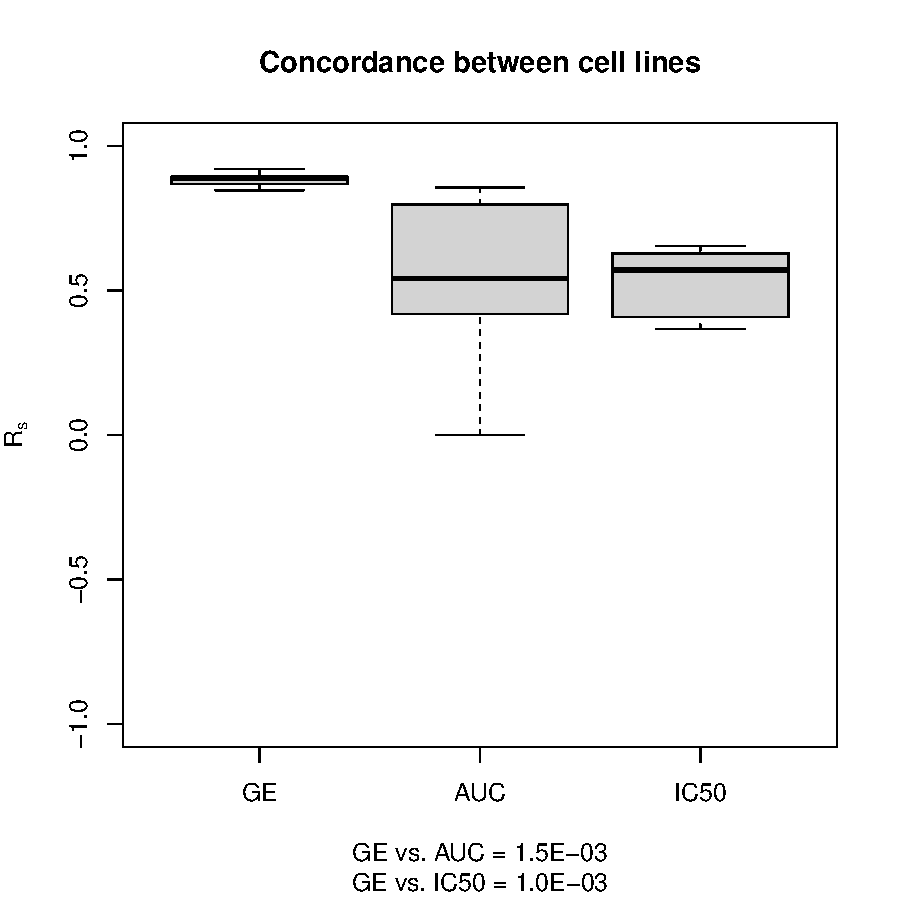
\includegraphics{PharmacoGx-fig2}
\end{center}
\label{fig:one}
\end{figure}

%------------------------------------------------------------
\subsection{Query the Connectivity Map}
%------------------------------------------------------------

The second case study illustrates the analysis of a perturbation type datasets, where the changes in cellular molecular profiles are compared before and after administering a compound to the cell line. Of these datasets, we have currently curated and made available for download the Connectivity Map (CMAP) dataset \cite{lamb_connectivity_2006}. \\

For this case study, we will recreate an analysis from the paper by Lamb et al., in which a known signature for HDAC inhibitors \cite{glaser_gene_2003} is used to recover drugs in the CMAP dataset that are also known HDAC inhibitors. For this example, the package includes this signature, already mapped to the gene level, and it can be loaded by calling \textit{data(HDAC\_genes)}.

Once again, we load the dataset, downloading it if needed using \textit{downloadPSet}. We then recreate drug signatures for each drug using the function \textit{drugPerturbationSig} to preform statistical modelling of the transcriptomic response to the application of each drug. We then compare the observed up-regulated and down-regulated genes to a the known HDAC signature, using the GSEA connectivity score to determine the correlation between the two signatures. 

\begin{Schunk}
\begin{Sinput}
>   library(PharmacoGx)
>   require(xtable)
>   data(CMAPsmall)
>   drug.perturbation <- drugPerturbationSig(CMAPsmall, mDataType="rna")
>   data(HDAC_genes)
>   res <- apply(drug.perturbation[,,c("tstat", "fdr")],
+                2, function(x, HDAC){ 
+ 	    return(connectivityScore(x=x, 
+ 	                             y=HDAC[,2,drop=FALSE], 
+ 	                             method="gsea", nperm=100))
+ 	}, HDAC=HDAC_genes)
>   rownames(res) <- c("Connectivity", "P Value")
>   res <- t(res)
>   res <- res[order(res[,1], decreasing=T),]
>   xtable(res, 
+     caption='Connectivity Score results for HDAC inhibitor gene signature.')
\end{Sinput}
% latex table generated in R 3.2.2 by xtable 1.7-4 package
% Wed Nov 11 23:45:28 2015
\begin{table}[ht]
\centering
\begin{tabular}{rrr}
  \hline
 & Connectivity & P Value \\ 
  \hline
vorinostat & 0.94 & 0.00 \\ 
  alvespimycin & 0.88 & 0.00 \\ 
  acetylsalicylic acid & 0.00 & 1.00 \\ 
  rosiglitazone & -0.71 & 0.00 \\ 
  pioglitazone & -0.73 & 0.09 \\ 
   \hline
\end{tabular}
\caption{Connectivity Score results for HDAC inhibitor gene signature.} 
\end{table}\end{Schunk}
As we can see, the known HDAC inhibitor Varinostat has a very strong connectivity score, as well as a very high significance as determined by permutation testing, in comparison to the other drugs, which score poorly. 

This example serves as a validation of the method, and demonstrates the ease with which drug perturbation analysis can be done using \textit{PharmacoGx}. While in this case we were matching a drug signature with a drug class signature, this method can also be used in the discovery of drugs that are anti-correlated with known disease signatures, to look for potential new treatments and drug repurposing.


%------------------------------------------------------------
\section{Estimating Drug Sensitivity Measures}
%------------------------------------------------------------ 
\textit{PharmacoGx} includes functions to calculate estimated AUC (Area Under
drug response Curve) and IC50 values from drugs dose response experiments that
measure cell viability after applications of varying concentrations of drug.
Additionally, these measures are recomputed for every \textit{sensitivity}
\textit{PharmacoSet} we create and included alongside any measures published
with the original data. The AUC measures originally published are labelled as \textit{auc\_published}, while the recomputed measures are labelled as \textit{auc\_recomputed}, and likewise for the IC50.

While the \textit{PharmacoSets} already contain the recomputed data, the AUC and IC50 can be calculated for arbitrary data using the \textit{computeIC50} and \textit{computeAUC} functions.  

%------------------------------------------------------------
\subsection{Curve Fitting}
%------------------------------------------------------------ 
While AUC can be numerically calculated without curve fitting, to estimate the IC50 a drug dose response curve must be fit to the data.The dose-response curves are fitted to the equation
$$y = \frac{1}{1+(\frac{x}{IC50})^{HS}}$$
where $y = 0$ denotes death of all infected cells, $y = y(0) = 1$ denotes no effect of the drug dose, $IC50$ is the concentration at which viability is reduced to half of the viability observed in the presence of an arbitrarily large concentration of drug, and $HS$ is a parameter describing the cooperativity of binding. $HS < 1$ denotes negative binding cooperativity, $HS = 1$ denotes noncooperative binding, and $HS > 1$ denotes positive binding cooperativity. The parameters of the curves are fitted using the least squares optimization framework.


%------------------------------------------------------------
\section{Gene-Drug Association Modelling}
%------------------------------------------------------------ 
\textit{PharmacoGx} provides methods to model the association between drugs and molecular data such as transcriptomics, genomics and proteomics. 
\textit{Sensitivity} studies allow the discovery of molecular features that improve or inhibit the sensitivity of cell lines to various compounds, by looking at the association between the expression of the feature and the response towards each compound. This allows the selection of drugs to be tailored to each specific patient based on the expressed known sensitivity biomarkers. The function \textit{drugSensitivitySig} models these associations.\\

\textit{Perturbation} studies on the other hand look at the molecular profiles of a cell before and after application of a drug, and therefore can characterize the action of a drug on the molecular level. It is hypothesized that drugs which act to down-regulate expression of known disease biomarkers would be effective in reversing the cell from a diseased to healthy state. The function \textit{drugPerturbationSig} models the molecular profiles of drugs tested in a \textit{perturbation} dataset.

%------------------------------------------------------------
\subsection{Sensitivity Modelling}
%------------------------------------------------------------ 
The association between molecular features and response to a given drug is modelled using a linear regression model adjusted for tissue source: 
$$Y = \beta_{0} + \beta_{i}G_i + \beta_{t}T$$
where $Y$ denotes the drug sensitivity variable, $G_i$ and $T$ denote the expression of gene i and the tissue source respectively, and $\beta$s are the regression coefficients. The strength of gene-drug association is quantified by $\beta_i$, above and beyond the relationship between drug sensitivity and tissue source. The variables Y and G are scaled (standard deviation equals to 1) to estimate standardized coefficients from the linear model. Significance of the gene-drug association is estimated by the statistical significance of $\beta_i$ (two-sided t test). P-values are then corrected for multiple testing using the false discovery rate (FDR) approach.\\

As an example of the efficacy of the modelling approach, we can model the significance of the association between two drugs and their known biomarkers in CCLE. We examine the association between drug \textit{17-AAG} and gene \textit{NQO1}, as well as drug \textit{PD-0325901} and gene \textit{BRAF}:

\begin{Schunk}
\begin{Sinput}
>   data(CCLEsmall)
>   features <- c(rownames(featureInfo(CCLEsmall, "rna"))[
+                           which(featureInfo(CCLEsmall,
+                                             "rna")$Symbol == "NQO1")],
+                 rownames(featureInfo(CCLEsmall, "rna"))[
+                           which(featureInfo(CCLEsmall,
+                                             "rna")$Symbol == "BRAF")])
>   sig <- drugSensitivitySig(pSet=CCLEsmall, 
+                             mDataType="rna", 
+                             drugs=c("PD-0325901", "17-AAG"), 
+                             features=features, 
+                             sensitivity.measure="auc_published", 
+                             molecular.summary.stat="median", 
+                             sensitivity.summary.stat="median")
>   xtable(sig[,,"pvalue"], caption='P Value of Gene-Drug Association')
\end{Sinput}
% latex table generated in R 3.2.2 by xtable 1.7-4 package
% Wed Nov 11 23:45:32 2015
\begin{table}[ht]
\centering
\begin{tabular}{rrr}
  \hline
 & PD-0325901 & 17-AAG \\ 
  \hline
ENSG00000181019\_at & 0.00 & 0.00 \\ 
  ENSG00000157764\_at & 0.00 & 0.18 \\ 
   \hline
\end{tabular}
\caption{P Value of Gene-Drug Association} 
\end{table}\end{Schunk}

%------------------------------------------------------------
\subsection{Perturbation Modelling}
%------------------------------------------------------------ 
The molecular response profile of a given drug is modelled as a linear regression model adjusted experimental batch effects, cell specific differences, and duration of experiment to isolate the effect of the concentration of the drug applied.: 
$$G = \beta_{0} + \beta_{i}C_i + \beta_{t}T + \beta_{d}D + \beta_{b}B$$
where $G$ denotes the molecular feature expression (gene), $C_i$ denotes the concentration of the compound applied, $T$ the cell line identity, $D$ denotes the duration of the experiment,  $B$ denotes the experimental batch, and $\beta$s are the regression coefficients. The strength of feature response is quantified by $\beta_i$. % CHECK THE NEXT SENTENCE
The variables $G$ and $C$ are scaled (standard deviation equals to 1) to estimate standardized coefficients from the linear model. Significance of the gene-drug association is estimated by the statistical significance of $\beta_i$ (two-sided t test). P-values are then corrected for multiple testing using the false discovery rate (FDR) approach.


%------------------------------------------------------------
\section{Connectivity Scoring}
%------------------------------------------------------------ 
The package also provides two methods for quantifying the similarity between two molecular signatures of the form returned by \textit{drugPerturbationSig} and \textit{drugSensitivitySig}, or a set of up and down regulated genes as part of a disease signature. 
The two methods are the \textit{GSEA} method as introduced by Subramanian et at \cite{subramanian_gene_2005}, and \textit{GWC}, a method based on a weighted Spearman correlation coefficient. Both methods are implemented by the \textit{connectivityScore} function.

%------------------------------------------------------------
\subsection{GSEA}
%------------------------------------------------------------ 

The \textit{GSEA} method is implemented to compare a signature returned by \textit{drugPerturbationSig} with a known set of up and down regulated genes in a disease state. For the disease signature, the function expects a vector of features with a value, either binary (1, -1) or continuous, where the sign signifies if the gene is up or down regulated in the disease. The names of the vector are expected to be the feature names, matching the feature names used in the drug signature. The function then returns a GSEA score measuring the concordance of the disease signature to the drug signature, as well as an estimated P-Value for the significance of the connectivity determined by permutation testing. 

%------------------------------------------------------------
\subsection{GWC}
%------------------------------------------------------------ 

The GWC method (Genome Wide Correlation) is implemented to compare two signatures of the same length, such as two drug signatures returned by \textit{drugPerturbationSig}. The score is a Spearman correlation weighted by the normalized negative logarithm significance of each value. The normalization is done so that datasets of different size can be compared without concern for lower p-values in one dataset due to larger sample sizes. 

More precisely, take $X_i$ and $Y_i$ to be the ranks of the first and second set of data respectively, and $Px_i$, $Py_i$ to be the p-values of those observations. The weight for each pair of observations is:
$$Wx_i = \frac{-\log_{10}(Px_i)}{\sum_{i}-\log_{10}(Px_i)}$$
$$Wy_i = \frac{-\log_{10}(Py_i)}{\sum_{i}-\log_{10}(Py_i)}$$
$$W_i = Wx_i + Wy_i$$

If we further define the weighted mean as follows:
$$ m(X;W) = \frac{\sum_i W_i X_i}{\sum_i{W_i}}$$
Then the weighted correlation is given by:
$$ cor(X,Y,W) = \frac{\frac{\sum_i W_i (X_i - m(X;W))(Y_i - m(Y,W))}{\sum_i W_i}}{\sqrt{(\frac{\sum_i W_i (X_i - m(X;W))^2}{\sum_i W_i})(\frac{\sum_i W_i (Y_i - m(Y;W))^2}{\sum_i W_i})}}$$

This correlation therefore takes into account not only the ranking of each feature in a signature, but also of the significance of each rank.

%------------------------------------------------------------
\section*{Session Info}
%------------------------------------------------------------ 

This Vignette was generated with the following R version and packages loaded:

\begin{itemize}\raggedright
  \item R version 3.2.2 (2015-08-14), \verb|x86_64-apple-darwin13.4.0|
  \item Locale: \verb|en_CA.UTF-8/en_CA.UTF-8/en_CA.UTF-8/C/en_CA.UTF-8/en_CA.UTF-8|
  \item Base packages: base, datasets, graphics, grDevices, methods,
    parallel, stats, utils
  \item Other packages: Biobase~2.28.0, BiocGenerics~0.15.6,
    PharmacoGx~1.1.0, xtable~1.7-4
  \item Loaded via a namespace (and not attached): bitops~1.0-6,
    caTools~1.17.1, cluster~2.0.3, digest~0.6.8, downloader~0.4,
    gdata~2.17.0, gplots~2.17.0, gtools~3.5.0, igraph~1.0.1,
    KernSmooth~2.23-15, limma~3.25.15, magrittr~1.5, marray~1.47.1,
    piano~1.8.2, RColorBrewer~1.1-2, relations~0.6-5, sets~1.0-15,
    slam~0.1-32, tools~3.2.2
\end{itemize}
\bibliographystyle{plain}
\bibliography{pharmacogx}

\end{document}
